\section{Architektur des Osmocom Systems}


\subsection{Was ist OsmoNITB}
Bei OsmoNITB handelt es sich um ein freies Softwarepacket aus dem Osmocom-Baseband-Projekt. Dessen Zweck ist das Aufspannen und Betreiben eines GSM/ GPRS-Netzes mittels nachgebauter Implementierungen des GSM-Protokolls. OsmoNITB bringt hierfür alle erforderlichen Bestandteile, die sich tiefer im Netz als die Basisstation (BTS) befinden. OsmoNITB übernimmt hierbei die Kommunikation mit der Basisstation. Dies geschieht über das A-bis-Interface, einer standardisierten Schnittstelle für den Datenaustausch zwischen Basisstation und Basisstation-Controller (Base Station Controller, BSC), welches selbst Bestandteil dieses Pakets ist. Neben diesen existieren noch folgende weitere Bestandteile:




\begin{itemize}
\item MSC/VLR\\
\item SMSC\\
\item EIR\\
\item HLR/AUC\\
\end{itemize}



\begin{figure}[h]
    \centering
    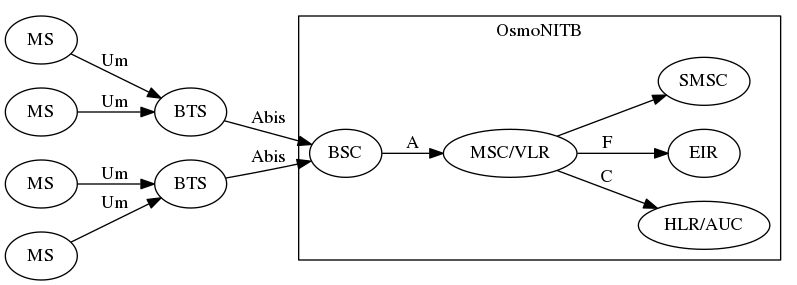
\includegraphics[width=10cm]{includes/osmonitb}
    \caption{GSM Systemarchitektur mit OsmoNITB}
	\label{fig:osmonitb}
\end{figure}






\subsection{Funktion der einzelnen Module}




\begin{itemize}

\item \textbf{BSC}\\
Hierbei handelt es sich wie bereits oben erwähnt um den Basisstationcontroller. Er überwacht eine Mobilfunkverbindung und regelt die Leistung nach. Zudem lösst er einen Zellenwechsel, dem sogenannten Handover aus. OsmoNITB nutzt hierzu die freie Implementierung OpenBSC.  

 
\item \textbf{MSC/VLR}\\
Die Mobile-service switching center stellt im GSM/GPRS-Netz die Vermittlungsstelle dar. Sie übernimmt die Anrufverwaltung, die Verwaltung der Authentifizierung und innerhalb eines kommerziellen Netzes auch die Gebührenerfassung. Das Visitor Location Register (VLR) würde zudem, die jeweilige Basisstation unter der ein Endgerät eingebucht ist oder zuletzt war, verwalten. Sie kennt damit den Ort des Mobilfunknutzers. Unser Projekt wird jedoch nur mit einer Basisstation durchgeführt, weshalb kein Handover nötig ist. Damit verbleibt das Mobiltelefon nur in einer Location. 


\item \textbf{SMSC}\\
Der SMSC ist ein Server für SMS-Dienste. Er kümmert sich um die Verarbeitung von Textmitteilungen. Hierunter fällt beispielsweise die Speicherung, Weiterleitung von SMS. Sie wird im weiteren Projektverlauf nicht benötigt.


\item \textbf{EIR}\\
Dies ist ein optionales Modul und wird nicht zwingend für den Betrieb eines GSM-Netzes benötig. Dabei handelt es sich um ein Equipment Identity Register (EIR). Hier werden die weltweit eindeutigen Seriennummern der Mobilgeräte (IMEI, International Mobile Equipment Identity) gespeichert. Ziel dieser Datenbank ist ein Sperren verlorener oder gestohlener Endgeräte zu ermöglichen. Auch sie wird in diesen Projekt nicht benötigt. Zudem verwenden auch im kommerziellen Betrieb nur wenige Mobilfunkbetreiber dieses, da die IMEIs oftmals verändert werden können und die Datenbank damit wirkungslos ist.  


\item \textbf{HLR/AUC}\\
HLR steht für Home Location Register und bildet die Datenbank in der die Nummer eine Mobiltelefons zu dessen eindeutigen Identifiers, der IMSI (International Mobile Subscriber Identity), hinterlegt ist. Zudem wird hier die TMSI aufgelöst. Eine temporäre IMSI, die den Nutzer eines Mobilgeräts durch Zuweisen einer veränderlichen Identifiers, besser vor Tracking schützen soll. Das Authentification Center (AUC) ist die Authentifizierungszentrale und damit der Ort, an dem der Authentifizierungsschlüssel Ki abgelegt ist. Hier wird die Authentifizierung der SIM-Karte gegenüber dem Mobilfunknetz durchgeführt. 


\end{itemize}


OsmoNITB implementiert damit das Network Switching Subsystem (NSS), aber mit dem BSC auch Teile des Base Station Subsystems (BSS). Das NSS ist hierbei der Teil der inneren Infrastruktur des Neztes, welches sich mit der Verwaltung von Mobilgeräten und Gesprächen beschäftigt. Das BSS hingegen kümmert sich im wesentlichen nur um die Verwaltung und Belegung der Funkschnittstelle.


\subsection{Funktionsweise von OsmoNITB}

In der Standardeinstellung von OsmoNITB werden Steuerungssignale von der BTS an diese weitergereicht, während die Gesprächsdaten mit Hilfe des verbindungslosen Protokoll UDP direkt an die Ziel-BTS gerichtet werden. Dazu sendet OsmoNITB in Form einer A-bis-Meldung einen Lauschbefehl an die Ziel-BTS. Eine Schicht höher wird dieses als Multimedia Protokoll RTP interpretiert. In unseren Projekt wurde die Einstellung „RTP proxy mode“ verwendet. Dies bewirkt, dass die RTP-Daten zuerst von OsmoNITB registriert werden und von dieser ausgehend nochmals an die Ziel-BTS versendet werden. Dies ist notwendig, da wir nur eine BTS betreiben, die zugleich Start-BTS und Ziel-BTS ist. Damit wird erreicht, dass dennoch ein RTP-Datenstrom detektierbar ist. Nachfolgendes Bild zeigt den prinzipiellen Aufbau eines derartigen Aufbaus:



\begin{figure}[h]
    \centering
    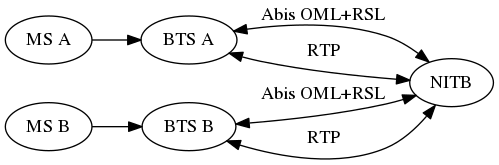
\includegraphics[width=8cm]{includes/osmonitb_rtp_proxy}
    \caption{OsmoNITB mit RTP proxy mode}
	\label{fig:osmonitb2}
\end{figure}


Weiterhin läuft auf unseren System die Telefonanlage Asterisk. Sie ist mittels Osmocom-Sip-Connector an OsmoNITB angeschlossen. Dieser generiert aus dem MNCC-Datenstrom aus OsmoNITB einen SIP-Datenstrom (Session Initiation Protocol).